\documentclass{article}
\usepackage[a4paper]{geometry}
\usepackage{bookmark}
\usepackage{amsmath,amsfonts,amsthm,amssymb,mathtools}
\usepackage[italian]{babel}
\usepackage{graphicx}
\usepackage{multirow}
\title{\Huge{Pendolo fisico}}
\author{\huge{Giosué Aiello, Domenico Fenili, Francesco Sermi}}
\date{14 Novembre 2023}

\begin{document}

\maketitle
\pagebreak
\tableofcontents
\pagebreak

\section{Scopo dell'esperienza}
Lo scopo di questa esperienza è quello di misurare il periodo di un pendolo fisico in funzione della distanza del perno di rotazione dal centro di massa.

\section{Cenni teorici}

\begin{figure}[h!]
	\centering
	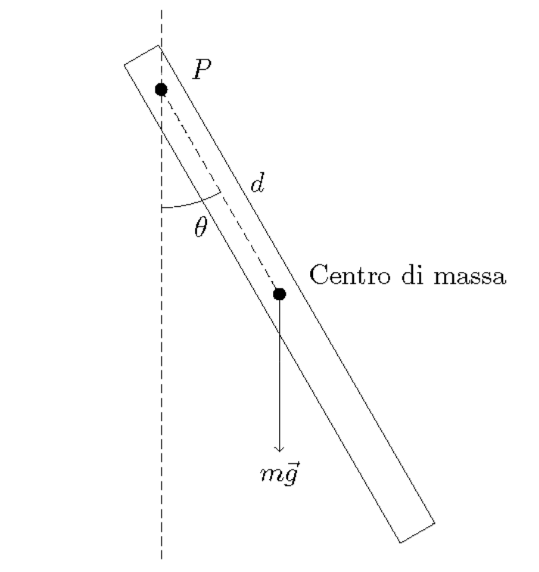
\includegraphics[scale=0.35]{pendolo_fisico.png}
	\caption{Schema del nostro apparato sperimentale}
	\label{fig:schema_pendolo}
\end{figure}
\par\smallskip\noindent Un oggetto fissato ad un punto di sospensione $P$ (che dista $d$ dal centro di massa) e soggetto alla gravità costituisce un pendolo fisico. Se questo corpo viene spostato di un angolo $\theta$ dalla sua posizione di equilibrio, il momento torcente della forza di gravità (rispetto al punto di sospensione $P$) vale:
\begin{equation}
	\tau = -mgd\sin{\theta}
\end{equation}
che, per $\theta << 10^\circ - 15^\circ$ possiamo esprimere $sin(\theta)$ utilizzando la formula di espansione in serie di Taylor al primo ordine:
\begin{equation*}
	\sin{\theta} = \sum_{n = 0}^{+\infty} \frac{(-1)^n}{(2n+1)!}\theta^{2n+1} = \theta + o(\theta^3) \approx \theta
\end{equation*}
Pertanto possiamo riscrivere il momento torcente della forza di gravità come:
\begin{equation*}
	\tau = -mgd\theta
\end{equation*}
E per la seconda equazione cardinale si ha che:
\begin{equation}
	\tau = \frac{dL}{dt}
\end{equation}
e sapendo che il momento angolare di un pendolo fisico risulta essere pari a $L = I\omega$ e $\omega = \frac{d\theta}{dt}$ si ha che:
$$
	\tau = \frac{dL}{dt} = I\frac{d}{dt} \left(\frac{d\theta}{dt} \right) = I\frac{d^2 \theta}{dt^2}
$$
Combinando la $(1)$ e la $(2)$:
\begin{equation}
	I\frac{d^2 \theta}{dt^2} = -mgd\theta \implies \frac{d^2 \theta}{dt^2} + \frac{mgd}{I}\theta = 0 
\end{equation}
Siamo dinanzi ad un'equazione differenziale di secondo ordine a coefficienti costanti omogenea di un moto armonico con pulsazione e periodo di oscillazione dati da:
$$\omega_0 = \sqrt{\frac{mgd}{I}} \, \, \, \, \, \, T_0 = 2\pi\sqrt{\frac{I}{mgd}}$$
Utilizzando il teorema degli assi paralleli, possiamo concludere che il momento di inerzia dell'oggetto fisico risulta essere:
$$
	I = I_{cm} + md^2 = \frac{ml^2}{12} + md^2
$$
Possiamo quindi riscrivere la formula nella seguente maniera:
\begin{equation}
	T(d) = \sqrt{\frac{m(l^2 + d^2)}{mgd}} = \sqrt{\frac{\frac{l^2}{12} + d^2}{gd}}
\end{equation}
\section{Apparato sperimentale e strumenti}

\begin{itemize}
	\item Strumenti 
	\begin{itemize}
		\item Metro a nastro, risoluzione $0. 1 cm$;
		\item Calibro ventesimale, risoluzione $0.05 mm$;
		\item Cronometro, risoluzione $0.01 s$
	\end{itemize}
	\item Materiali
	\begin{itemize}
		\item Asta metallica forata;
		\item Un supporto di sospensione;
	\end{itemize}
\end{itemize}

\section{Descrizione delle misure}

--Completare

\section{Analisi dei dati}

\begin{table}[h!]
	\hspace{-0.1\textwidth}	
	\begin{minipage}{0.1\textwidth}
		\centering
		\begin{tabular}{ | r | c | c | }
			\hline
			\multirow{2}{5em}{Numero prova}& $\tau (s)$ & $d (cm) $ \\
			& $\pm 0.01$ & $\pm 0.1$ \\
			\hline
			1 & 16.09 & \multirow{7}{1em}{$95.0$} \\ \cline{1-2}
			2 & 15.90 & \\	\cline{1-2}
			3 & 	15.73 & \\	\cline{1-2}
			4 &	15.93 & \\	\cline{1-2}
			5 &	15.89 & \\	\cline{1-2}
			6 &	15.67 & \\	\cline{1-2}
			7 &	16.00 & \\	\cline{1-2}
			\hline
		\end{tabular}
	\end{minipage}
	\hspace{0.3\textwidth}
	\begin{minipage}{0.1\textwidth}
		\centering
		\begin{tabular}{ | r | c | c | }
    		\hline
    		\multirow{2}{5em}{Numero prova} & $\tau$ (s) & $d$ (cm) \\
    		& $\pm 0.01$ & $\pm 0.1$ \\
    		\hline
    		1 & 15.31 & \multirow{7}{*}{85.0} \\ \cline{1-2}
    		2 & 15.42 & \\ \cline{1-2}
    		3 & 15.30 & \\ \cline{1-2}
    		4 & 15.56 & \\ \cline{1-2}
    		5 & 15.29 & \\ \cline{1-2}
    		6 & 15.50 & \\ \cline{1-2}
    		7 & 15.53 & \\ \cline{1-2}
    		\hline
		\end{tabular}
	\end{minipage}
	\hspace{0.3\textwidth}
	\begin{minipage}{0.1\textwidth}
		\centering
		\begin{tabular}{ | r | c | c | }
    		\hline
    		\multirow{2}{5em}{Numero prova} & $\tau$ (s) & $d$ (cm) \\
    		& $\pm 0.01$ & $\pm 0.1$ \\
    		\hline
    		1 & 15.75 & \multirow{7}{*}{75.0} \\ \cline{1-2}
    		2 & 15.66 & \\ \cline{1-2}
    		3 & 15.73 & \\ \cline{1-2}
    		4 & 15.61 & \\ \cline{1-2}
    		5 & 15.67 & \\ \cline{1-2}
    		6 & 15.80 & \\ \cline{1-2}
    		7 & 15.67 & \\ \cline{1-2}
    		\hline
		\end{tabular}
	\end{minipage}
\end{table}

\end{document}
